\documentclass[11pt]{extarticle}
\usepackage{mathtools}
\usepackage[a4paper, total={6in, 8.5in}, top=1in, bottom=1in, left=1in, right=1in]{geometry}
\usepackage{graphicx}
%\usepackage{subfig}
\usepackage{amssymb}
\usepackage{amsmath}
\usepackage{pythonhighlight}
\usepackage{pdfpages}
\usepackage[T1]{fontenc}
\usepackage[utf8]{inputenc}
\usepackage{fancyhdr}
\usepackage{pythonhighlight}
\usepackage{changepage}
\usepackage{slashbox}
\usepackage{floatrow}
\usepackage{listings}
\usepackage[hidelinks]{hyperref}
\usepackage{fontawesome}
\usepackage{subcaption}
\usepackage{color} %red, green, blue, yellow, cyan, magenta, black, white
\definecolor{mygreen}{RGB}{28,172,0} % color values Red, Green, Blue
\definecolor{mylilas}{RGB}{170,55,241}


\floatsetup[table]{capposition=top}

\sloppy
\definecolor{lightgray}{gray}{0.5}
\setlength{\parindent}{0pt}
\setlength{\headheight}{14pt}

\renewcommand{\headrulewidth}{.4mm} % header line width
\newcommand{\norm}[1]{\left\lVert#1\right\rVert}




\pagestyle{fancy}
\fancyhf{}
\fancyhfoffset[L]{-1cm} % left extra length
\fancyhfoffset[R]{-1cm} % right extra length
\rhead{\bfseries Kutay U\u{g}urlu 2232841}
\lhead{EE583 Homework 4}
\rfoot{}

\DeclarePairedDelimiter\ceil{\lceil}{\rceil}
\DeclarePairedDelimiter\floor{\lfloor}{\rfloor}

\author{Kutay U\u{g}urlu 2232841}

\begin{document}

\lstset{language=Matlab,%
    %basicstyle=\color{red},
    breaklines=true,%
    morekeywords={matlab2tikz},
    keywordstyle=\color{blue},%
    morekeywords=[2]{1}, keywordstyle=[2]{\color{black}},
    identifierstyle=\color{black},%
    stringstyle=\color{mylilas},
    commentstyle=\color{mygreen},%
    showstringspaces=false,%without this there will be a symbol in the places where there is a space
    numbers=left,%
    numberstyle={\tiny \color{black}},% size of the numbers
    numbersep=9pt, % this defines how far the numbers are from the text
    emph=[1]{for,end,break},emphstyle=[1]\color{red}, %some words to emphasise
    %emph=[2]{word1,word2}, emphstyle=[2]{style},    
}

\fancyfoot[C]{\thepage}
\title{\LARGE \LARGE EE583 Pattern Recognition HW4}

\maketitle{\LARGE}

\pagebreak


\section{Question 1}

\begin{center}
    \begin{figure}[h]
        \begin{tabular}{cc}
            \subfloat[]{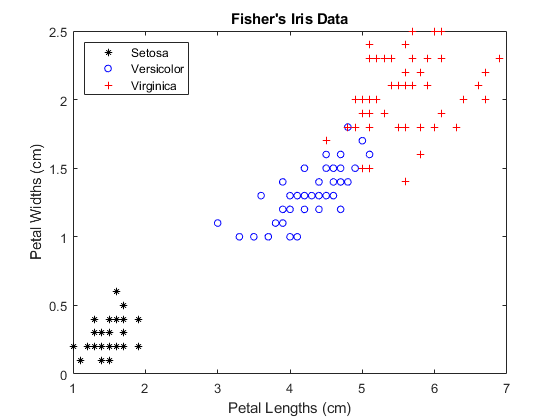
\includegraphics[width = 2in, height = 1.5in]{Q1_dist.png}} &
            \subfloat[]{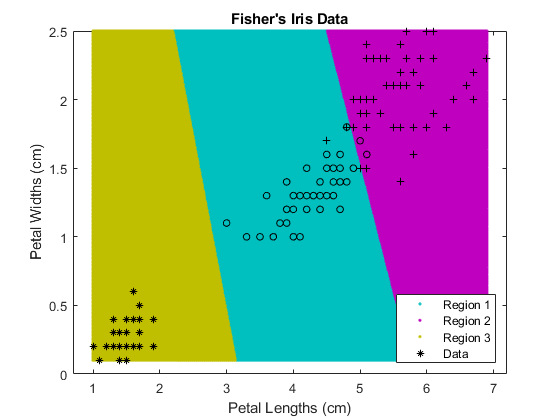
\includegraphics[width = 2in, height = 1.5in]{Q1_grid.png}}   \\
        \end{tabular}
        \caption{The data distribution and partitioning}
        \label{fig:q1fig}
    \end{figure}
\end{center}

\begin{center}
    \begin{figure}[h]
        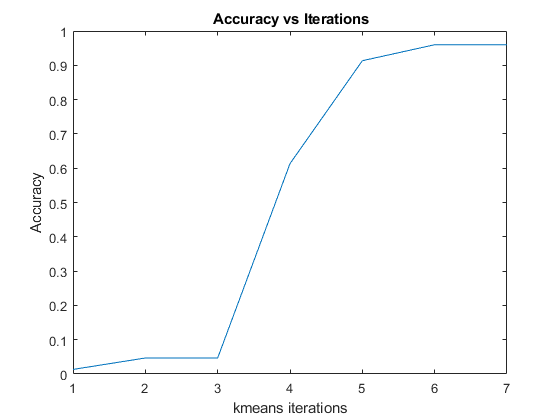
\includegraphics[width = 2in, height = 1.5in]{Q1_acc.png}
        \caption{classification success for different centroids}
        \label{fig:q1_2fig}
    \end{figure}
\end{center}

The centroids are manually set according to the approximate mean deduced from the data distribution plot. Initial centroids
can be found in \ref{subsec:Q1_code}. The accuracy is calculated in two steps. First, the confusion matrix is calculated, then the diagonal entries of it are added to obtain the true positive classifications. Finally, $Accuracy \triangleq \frac{\#TP}{\#Samples}$.
\\
Figure \ref{fig:q1_2fig} shows the accuracies of the iterations initialized with different centroids. Through careful centroid selection, the accuracy can be increased from 0.1 to 0.9647.

\pagebreak

\section{Question 2}

\begin{figure}[h]%
    \centering
    \begin{subfigure}{4cm}
        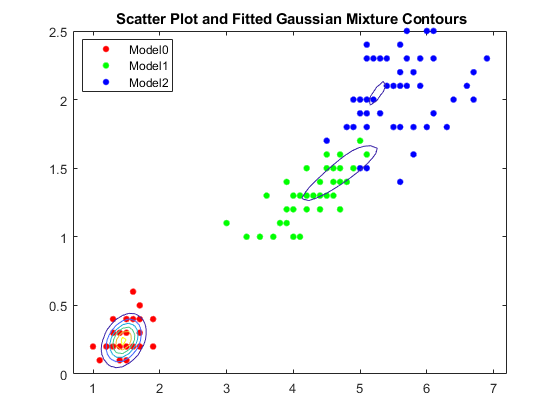
\includegraphics[width=\linewidth]{Q2.png}
        \caption{Case 1}\label{fig:random3}
    \end{subfigure}
    \qquad
    \begin{subfigure}{4cm}
        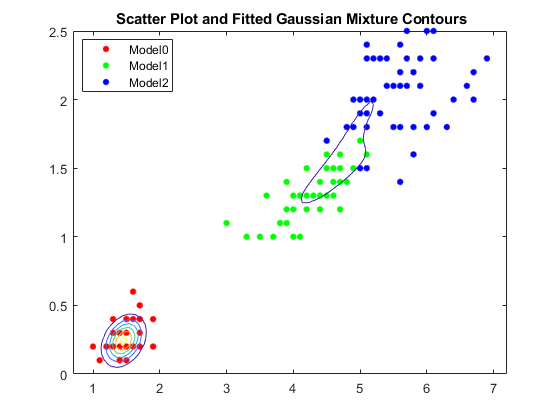
\includegraphics[width=4cm]{Q21.png}
        \caption{Case 2}\label{fig:random2}
    \end{subfigure}
    \caption{Gaussian Fits}%
    \label{fig:q2}%
\end{figure}

I have included 2 different versions of Gaussian fit to the feature vectors, due to the randomness of the algorithm. In Figure \ref{fig:random3}, I have observed 3 different Gaussian fits. However, the second trial resulted in algorithm fitting 2 different features to the same Gaussian distribution in Figure \ref{fig:random2}.

\section{Question 3}
\begin{figure}[h]
    \centering
    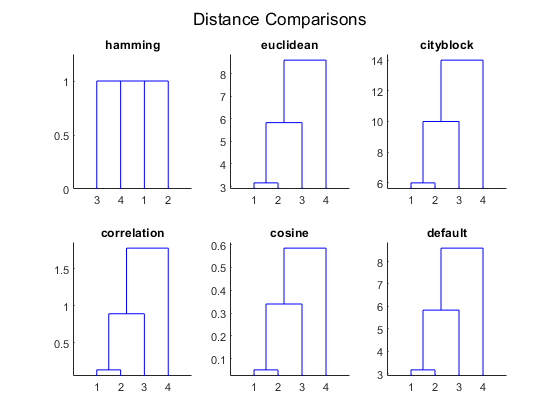
\includegraphics[width = 6.2in, height = 3in]{Q3.png}
    \caption{Dendrograms for different metrics}
    \label{fig:q3fig}
\end{figure}

All the metrics beside Hamming and Mahalanobis, resulted in similar dendrograms with easily noticeable difference in the distances in the relevant scales. However, distance calculated using Mahalanobis resulted in close numbers, hence even in
order of $10^{-8}$ the dendrogram presentation is not clear. Hamming distance calculate the percentage of different coordinates in the data matrix $X$. Since all rows of $X$ carries unique elements, Hamming metric resulted in $100\%$ for all off the feature vectors.

\pagebreak

\section{Question 4}

\subsection{Precomputed clustering}
\begin{center}
    \begin{figure}[h]
        \begin{tabular}{cc}
            \subfloat[]{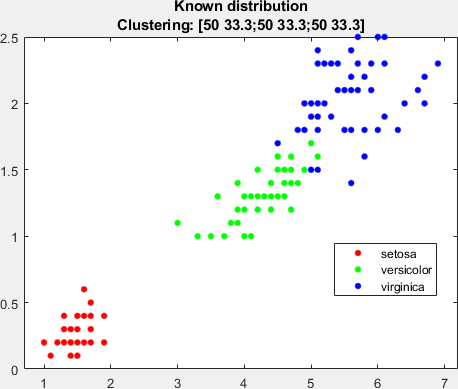
\includegraphics[width = 2in, height = 1.5in]{Q4_8.png}} &
            \subfloat[]{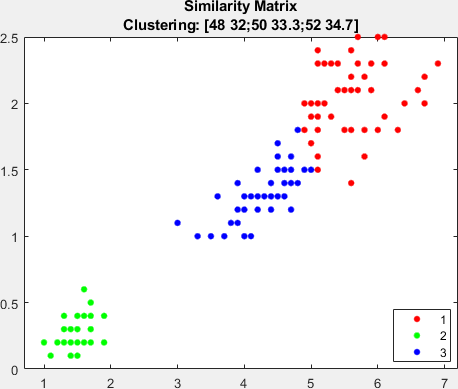
\includegraphics[width = 2in, height = 1.5in]{Q4_7.png}}   \\
        \end{tabular}
        \caption{Clustering for different cases}
        \label{fig:q40fig}
    \end{figure}
\end{center}

\subsection{Laplacian Matrix Normalization}
\begin{center}
    \begin{figure}[h]
        \begin{tabular}{cc}
            \subfloat[]{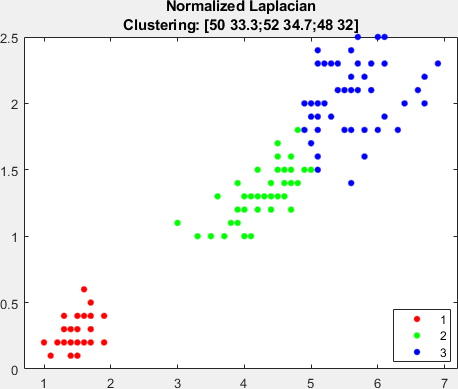
\includegraphics[width = 2in, height = 1.5in]{Q4_6.png}} &
            \subfloat[]{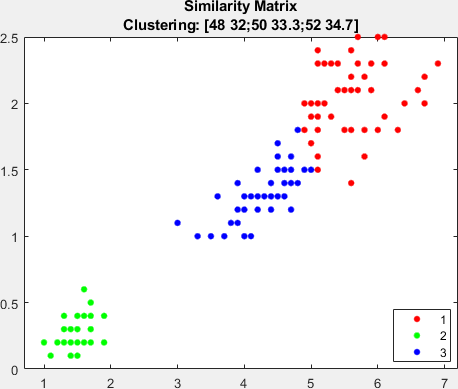
\includegraphics[width = 2in, height = 1.5in]{Q4_5.png}}   \\
        \end{tabular}
        \caption{Clustering for different cases}
        \label{fig:q41fig}
    \end{figure}
\end{center}
\vspace*{-1cm}
Using unnormalized Laplacian matrix increased the number of misclassifications.

\pagebreak

\subsection{Distance Metrics}
\begin{center}
    \begin{figure}[h]
        \begin{tabular}{cc}
            \subfloat[]{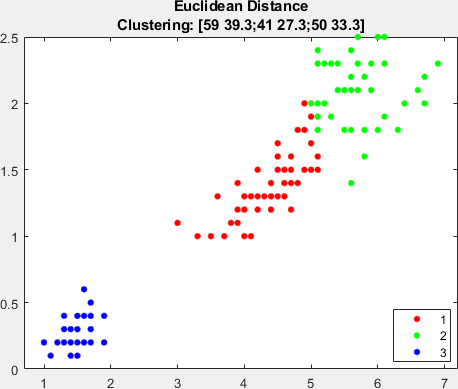
\includegraphics[width = 2in, height = 1.5in]{Q4_4.png}} &
            \subfloat[]{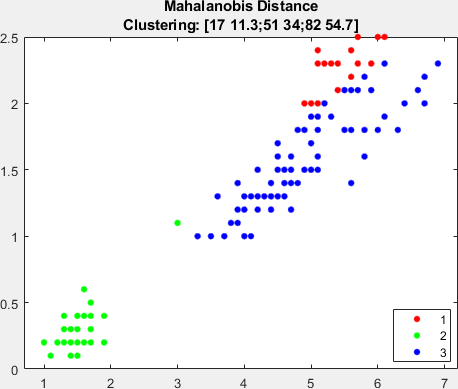
\includegraphics[width = 2in, height = 1.5in]{Q4_3.png}}   \\
        \end{tabular}
        \caption{Clustering for different cases}
        \label{fig:q42fig}
    \end{figure}
\end{center}
When the clustering is based on Mahalanobis distance metric, the accuracy gets bad. Since, it takes into distances to the mean of normalized distribution. On the other hand, Euclidean metrics finds the neighborhood relationship simply calculating the distance between data point on 2 dimensional feature space. Hence, the result is closer to the real distribution.

\subsection{Kernel Scale}
\begin{center}
    \begin{figure}[h]
        \begin{tabular}{cc}
            \subfloat[]{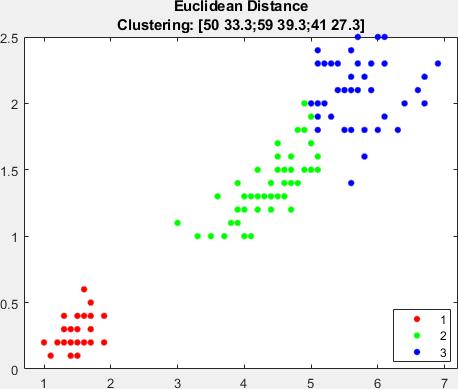
\includegraphics[width = 2in, height = 1.5in]{Q4_2.png}} &
            \subfloat[]{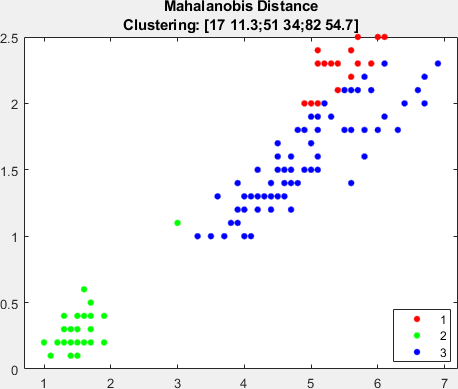
\includegraphics[width = 2in, height = 1.5in]{Q4_1.png}}   \\
        \end{tabular}
        \caption{Clustering for different cases}
        \label{fig:q43fig}
    \end{figure}
\end{center}

Kernel scale parameter is used to scale the distance in the pairwise similarity definition:

\begin{equation}
    \label{eq:similarity}
    S_{i,j} = e^{-(\frac{D_{i,j}}{\sigma})^2}
\end{equation}

According to Eqn. \ref{eq:similarity}, the similarity of 2 data points is exponentially proportional to the similarity. Hence, using a larger kernel scale will result in increased similarity in further data points. This is exactly what is observed in Figure \ref{fig:q43fig}. Kernel scale of 15 resulted in further points to be classified in the same cluster, hence caused misclassifications.

\pagebreak
\section{APPENDIX}
The code given in this section is shared \href{https://github.com/kutay-ugurlu/Pattern-Recognition/tree/master/HW4}{@\faGithubSquare}.
\subsection{Q1}\label{subsec:Q1_code}
\lstinputlisting{HW4_Q1.m}
\pagebreak
\subsection{Q2} \label{subsec:Q2_code}
\lstinputlisting{HW4_Q2.m}
\pagebreak
\subsection{Q3}\label{subsec:Q3_code}
\lstinputlisting{HW4_Q3.m}
\pagebreak
\subsection{Q4}\label{subsec:Q4_code}
\lstinputlisting{HW4_Q4.m}
\end{document}